As described in section \ref{stressnstrain} Cauchy’s strain tensor is only valid for small deformations. This is a problem since only large deformations results in visual interesting effects. In section \ref{eqn:stiffnessmatrix} stiffness matrix is obtained from $V_{e}$, $B_{e}$ and $E$ which is all constant depending on the initial state of the tetrahedron. Due to large deformations during simulation time this stiffness matrix will become unvalued. M\"uller (referens) proposed a solution to this problem called Stiffness Warping. This method compensates the error by rotating the deformed tetrahedron back into its original coordinate frame. The rotation is found by forming the matrix A which is the non translation part of the mapping between the two tetrahedrons shown in equation.

\begin{equation}\label{eqn:stiffnessmatrix}
    A = [x_{1}-x_{0}, x_{2}-x_{0}, x_{3}-x_{0}][p_{1}-p_{0}, p_{2}-p_{0}, p_{3}-p_{0}]^{-1}
\end{equation}

A Gram-Schmidt method is used to extract the rotation matrix $R$  $A$  

\begin{figure}[h]
\centering
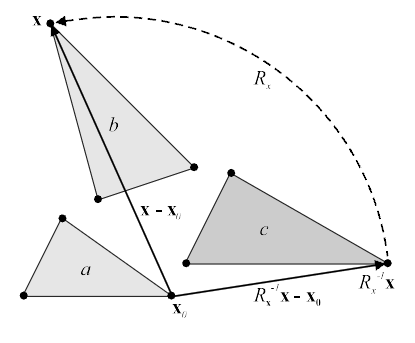
\includegraphics[width=.5\columnwidth]{figures/warpedstiffness.png}
\caption{}
\label{fig:4}
\end{figure}